
\documentclass[a4paper,twoside,12pt,compact]{article}
%\documentclass[a4paper,fontsize=12pt]{scrartcl}
\pagestyle{empty} % suppress page numbers

% set margins
%\usepackage[left=0.9cm,top=0.9cm,right=0.9cm,bottom=0.9cm,bindingoffset=0cm]{geometry}
\usepackage[left=1.1cm,top=1.1cm,right=1.1cm,bottom=1.1cm,bindingoffset=0cm]{geometry}

%%%%%%%%%
% fonts %
%%%%%%%%%

% use the Alegreya font
%\usepackage{Alegreya}
%\usepackage{AlegreyaSans}

% a times new roman clone
 \usepackage{times}

% true Times New Roman with XeLaTeX
%\usepackage{fontspec}
%\setmainfont{Times New Roman}

\usepackage[svgnames,hyperref]{xcolor}
\usepackage{url}
\usepackage{graphicx}

\usepackage{amsmath,amssymb,amsthm}
\usepackage{tikz}
\usetikzlibrary{shapes,arrows}
\usepackage[utf8]{inputenc}

%\usepackage[backend=biber,style=authoryear, maxbibnames=10,url=false,doi=false]{biblatex}

% make bibliography a bit smaller if necessary
% \renewcommand*{\bibfont}{\footnotesize} 
% \footnotesize should be 10pt with a standard 12pt class, 
% see https://en.wikibooks.org/wiki/LaTeX/Fonts#Sizing_text

% \AtEveryBibitem{\clearfield{month}}
% \AtEveryCitekey{\clearfield{month}}

%\addbibresource{references.bib}

% Change  the spacing in the bibliography
\newlength{\bibitemsep}\setlength{\bibitemsep}{.1\baselineskip plus .05\baselineskip minus .05\baselineskip}
\newlength{\bibparskip}\setlength{\bibparskip}{0pt}
\newlength{\biblineskip}\setlength{\biblineskip}{11pt}

\let\oldthebibliography\thebibliography
\renewcommand\thebibliography[1]{%
  \oldthebibliography{#1}%
  \setlength{\parskip}{\bibitemsep}%
  \setlength{\itemsep}{\bibparskip}%
  \setlength{\baselineskip}{\biblineskip}%
}


\usepackage[english=british,threshold=15,thresholdtype=words]{csquotes}
%\SetCiteCommand{\parencite}
\newcommand{\parencite}[1]{\cite{#1}}
\newcommand{\textcite}[2]{\cite{#2}}

\newenvironment*{smallquote}
{\quote\small}
{\endquote}
\SetBlockEnvironment{smallquote}

\usepackage[%
unicode=true,
hyperindex=true,
bookmarks=true,
colorlinks=true, % change to false for final
pdfborder=0,
allcolors=DarkBlue,
% plainpages=false,
pdfpagelabels,
hyperfootnotes=true]{hyperref}

\usepackage{todonotes}

\author{}

\date{\today}

\begin{document}

\section*{C1. Project Description}
\label{sec:project-description}
% (Please upload a Project Description as detailed in the Instructions
% to Applicants in no more than 10 A4 pages and in the required
% format. Please refer to the Instructions to Applicants for detailed
% instructions on the required content and format of the Project
% Description.)

\subsection*{PROJECT TITLE}
% can differ from grant title and be longer 

\textbf{Live coding of complex flood simulations with uncertainty quantification}

\subsection*{AIMS AND BACKGROUND}

When systems are disrupted during environmental disasters (for example,
during floods, storm surges or tsunamis) information from
computational simulation is needed urgently to aid decision-making by
emergency services. This is not simply a matter of compute power but
requires insight from applied mathematics, software
engineering, human computer interaction, high performance computing
and data visualisation. All of these facets need to be tightly coupled
and {\bf tested in realistic  decision-making
scenarios} where decision makers collaborate with modelling experts. In
particular, a crucial aspect of advice provided from modellers to
decision makers is to {\bf properly quantify and communicate the
{uncertainty}} in predictions obtained by computer simulations.
This advice needs to be provided in a timely manner and in a context
where the computer support may vary dramatically due to
system outages.

We will address this grand challenge through a \emph{live programming}
approach to the development and deployment of software systems for
environmental simulation in the presence of uncertainty. We will
\textbf{develop} new `inundation models' (models of riverine floods,
storm surges and tsunamis) which use sparse grids and uncertainty
quantification to dramatically increase the speed and usefulness of
model predictions and their associated uncertainty. We will
\textbf{deploy} `live' distributed computing infrastructure to
\emph{rapidly prototype} the human interface to these new
environmental simulations and to transform the traditional,
batch-oriented workflow of environmental simulation into a highly
interactive one. Indeed live programming offers an unprecedented opportunity
for interactive parallel program performance evaluation and tuning.
We will \textbf{evaluate} team coordination and
decision-making in the presence of uncertainty through role-playing
scenarios of representative flood and tsunami situations. In these mock
field trials, we will record (both through instrumented system logs
and interviews with participants) the interaction patterns and
protocols of live programmed optimisation of the software modelling
systems. From a human-computer interaction (HCI) analysis of these
protocols, we will \textbf{identify} patterns in the interaction
states and transitions between those states which we will use to
iterate our software-system development.

Our vision is that using this approach, decision makers will be able
to examine many different environmental disaster scenarios in a short
space of time, even with computationally-expensive models. This will
enable them to develop an intuitive understanding of the uncertainty
relationships in the system---from uncertainties in input data through
to representations of uncertainty in model outputs. The importance of
this human-in-the-loop workflow is expressed by~\cite{pikeScience2009}
in the following quote: ``it is through the interactive manipulation
of a visual interface---the analytic discourse---that knowledge is
constructed, tested, refined and shared.''

Although the mathematical and computational tools we will employ in
this project are generalisable to any modelling workflow, our focus is
on specific application domains where (a) the model is
(computationally) complex, (b) uncertainty is significant and (c)
decisions are time-sensitive. Specifically, we will build interactive
interfaces for riverine floods, storm surge and tsunami modelling,
which exemplify these characteristics.

When uncertainty is included into a model, the 
essential dimensionality of the problem is increased markedly.  
New and more sophisticated techniques are then required to deal with the so called
`curse of dimensionality', where
the cost of computation increases exponentially with the dimension of
the problem. 

The mathematical component of this project will be based on new
developments combining reduced order models 
(such as sparse grids and reduced basis methods)
with uncertainty quantification.
Sparse grids~\parencite{BungartzGriebel2004} are known to
reduce the effects of the curse of dimensionality and 
recent work in our group has found new ways to incorporate gradient
information and multi-fidelity models into sparse grid
approximations~\parencite{deBaarHarding2015,Jakeman2015,deBaarRDM2015}.
We will extend this work to construct efficient techniques 
for incorporating uncertainty  information into 
storm surge-tsunami models. 
Reduced basis 
methods~\parencite{quarteroni2015reduced} provide an 
alternative approach for constructing reduced order 
models and will also be investigated.

Computational decision support systems for disaster management have
existed for many decades \parencite{wallaceDecision1985}, and
advances have been made both in incorporating
uncertainty \parencite{thompsonSocial2014,nealeNavigating2015}
and providing real-time interaction and
output~\parencite{yuSupport2006}. More recently, mixed-reality game
scenarios have been used to understand and optimise human-agent
collaboration for disaster response~\parencite{ramchurn2016human}. In
our project plan we will follow a similar approach and will employ
mock-game scenarios to examine and understand the nature of decision
making with expert modelling support. In a novel twist, we will run
these games together with live-coding optimisation and tuning of the
software system and the underlying computational platform. By
analysing the protocols of these live optimisations, we will
accumulate data to feed into redesign of the software interface and to
understand the time requirements and controls needed for the
computational platform.

\medskip
This project will provide the following discoveries and benefits:
\begin{enumerate}

\item a suite of interactive, real-time modelling tools for
  surge-tsunami flood disasters which combine high fidelity
  simulations (fine grids) with low fidelity (coarse grid) simulations
  to quantify uncertainty, optimised for human exploration

\item a `live software engineering' approach to the development,
  deployment and optimisation of these interactive software systems

\item models of group interaction scenarios for decision-making with
  expert modelling support; from these models, we will obtain  empirical estimates of
  the time constraints that such scenarios impose on software
  and computer system requirements and the live controls needed to run
  them effectively in volatile contexts

\item interactive information visualisation of simulation predictions
together with uncertainties
 

\end{enumerate}

This research is significant because it aims to unlock the power of
sophisticated computational simulation for \emph{interactive} use.
Although we concentrate our research on simulation support for
disaster response, the ultimate potential of this work is to
eventually empower domain experts from a broad range of areas to
better use the high-performance computing power which is now available
to them. We envision a future where performing a complex flood model
or disaster simulation is as interactive and \emph{alive} as flicking
through photos on a tablet.




\subsection*{ROLE OF PERSONNEL}
% - Summarise the role, responsibilities and contributions of each Chief Investigator (CI) and Partner Investigator (PI)
% - Summarise the roles and levels of involvement of other Participants, for example, technical staff, Research Associates and other personnel
% - Describe how each Participant will ensure they have the ‘time and capacity’ to undertake the proposed research, taking into account any other grants or roles that they hold.

%The personnel on this grant cover the key research areas discussed in
%the \emph{Research Project} section of this application:
%
%\begin{itemize}
%\item \textbf{Steve Roberts}: uncertainty quantification, sparse grids, flood
%  modelling
%\item \textbf{Markus Hegland}: sparse grids
%\item \textbf{Peter Strazdins}: sparse grids, distributed computing
%\item \textbf{Henry Gardner}: HCI, interfaces
%\end{itemize}

The personnel involved in this project will be the CIs Gardner,
Roberts, Strazdins and Hegland, 
%the PIs Jakeman and Debusschere, 
and
two Postdoctoral Research Associates and four PhD students.  This
project is split between the ANU Research School of Computer Science
(CI Gardner, CI Strazdins, one PDRA, two PhD students) the ANU
Mathematical Sciences Institute (CI Roberts, CI Hegland, one PDRA and
two PhD students).
%together will support from Sandia National Labs (PI
%Jakeman and PI Debusschere). 


CI Strazdins will be
responsible for the high performance and distributed computing
components of the project, based on his expertise in high performance
computing~\parencite{AliEtal2015,StrazdinsEtal2015,Ali11022016}.  
CI Strazdins has a 40\% research allocation. In 2017 he contribute of 20\% of his research time to the LE150100030, leaving sufficient research time to cover the proposed 20\% allocation to this project. 
%
CI Gardner will be responsible for the interactive computing and visual interface components of this project, based on
his expertise in HCI and visualisation~\parencite{martin2016intelligent,martin2015tracking,swift2014coding,swift2013visual,sorensen2010programming,swiftLive2016}.  CI Gardner has a 40\% research allocation. In 2017 he will have a potential contribution of 10\% of his research time to the LP160100624 which is presently under consideration, leaving sufficient research time to cover the proposed 20\% allocation to this project. 
%
CI Roberts will lead the inundation modelling, and
uncertainty quantification components, based on his expertise in
computational fluid dynamics and the use of sparse grid based
uncertainty quantification~\parencite{deBaarRDM2015,JakemanRoberts2013,anugamanual,nielsen2005hydrodynamic}.  
CI Roberts has a 40\% research allocation, with no current grant obligations,  leaving sufficient research time to cover the proposed 20\% allocation to this project. 
%
CI Hegland will be responsible for the
sparse grid and reduced model component of the project, based on his
extensive expertise in computational mathematics, in particular his
expertise in the analysis of the combination technique for sparse
grids~\parencite{AliEtal2015,HardingHLS2015,Ali11022016}. 
CI Hegland has a 60\% research allocation. In 2017 he contribute of 20\% of his research time to the DP150102345, and potentially 20\% contribution to LP160100624 leaving sufficient research time to cover the proposed 20\% allocation to this project. 

%PI Jakeman will provide expertise on uncertainty
%quantification techniques based on his extensive experience in
%applying such techniques to complex modelling 
%problems~\parencite{JakemanRoberts2013,jakemanNumerical2010,Jakeman2015}.  
%PI Debusschere will provide his extensive expertise in uncertainty
%quantification through to fault tolerant numerical solvers.

One post-doctoral fellow, to be situated in the
Research School of Computer Science (RSCS), will develop large
portions of the live programming tools and software interface which
will interact with the scientific models and will conduct experiments
on live scenarios where human actors mimic the interactions and
information flows involved in the group dynamics of disaster response
with simulation support. Due to the large skill set and responsibilities of 
this position it has been factored into the budget at level B3.
One possible candidate for this position is 
Dr Ben Swift who is currently a post doc in the RSCS and has work 
extensively in HCI and has collaborated extensively with CI Gardner, on work 
relevant to this project ~\parencite{martin2015tracking,martin2016intelligent,swiftLive2016,
swift2013visual,swift2014coding}.

The second post-doctoral fellow, to be
situated in the Mathematical Sciences Institute (MSI), 
will need to have a very different skills set to the computer 
science research fellow. This research fellow will develop
the numerical methods for computing sparse grid surrogates and reduced
basis models which will be used to efficiently propagate 
uncertainties in
model applications of tsunami and flood surge events. This 
position is budgeted at level B1 ( raising to B2 in year 3).
One possible candidate for this position is the current PhD 
student of CI Hegland, Mr Brendan Harding,  who has just 
submitted his PhD thesis on ``Fault Tolerant Computation of
Hyperbolic PDEs with the Sparse Grid Combination Technique''.
Mr Harding has collaborated with his supervisor, 
CI Hegland, along with CI Strazdins and CI Roberts, all
on work relevant to this project~\parencite{Ali11022016,AliEtal2015,deBaarHarding2015,
HardingHLS2015,StrazdinsEtal2015}.


The four PhD students will be split between the two departments---two
in RSCS and two in MSI, focusing on specific aspects of the project,
essentially aligned with the four CIs areas of responsibility.  In
RSCS, these will be the dynamic distributed computing infrastructure
and the development of live interfaces for data visualisation. In the
MSI, these will be the uncertainty quantification and the development
of numerical methods for the sparse grid technique, and the reduced
basis method, applied to our inundation model example.
We are requesting ARC funding for 2 PhDs, with funding for the other two PhDs coming 
from  Australian Postgraduate Awards.  Even though we have designated these 
PhD students as either being computer science or mathematics, the 
projects will be inter-disciplinary, with all four CIs being on the supervisory panels of 
each of the students. 

We anticipate being able to support a number of Honours projects in
computer science and mathematics during the course of this
project. Some of these projects will relate to the core mission of the
project detailed above, others will concentrate on related studies
with a view to achieving high-impact pure and applied research and
training young people for a career in the computing and mathematical
modelling disciplines.



\iffalse
\subsection*{RESEARCH PROJECT}
\fi
\subsection*{PROJECT QUALITY AND INNOVATION}

% - Describe how the research is significant and how it addresses an important problem
% - Describe how the Proposal meets the objectives of the Discovery Projects scheme
% - Describe how the anticipated outcomes will advance the knowledge base of the discipline and
%   how the Proposal aims and concepts are novel and innovative
% - Outline the conceptual framework, design and methods and demonstrate that these are
%   adequately developed, well integrated and appropriate to the aims of the Proposal. Include
%   research plans and proposed timelines
% - Detail what new methodologies or technologies will be developed in the course of the research
%   and how they will advance knowledge
% - Outline the feasibility of the project, in terms of design, budget and proposed timeline
% - If the rationale for some of the Proposal rests upon manuscripts that are still in the process of
%   being published, or on results of work that may not be available to assessors, include a
%   summary of the relevant work
% - Describe the expected outcomes and likely impact of the proposed research
% - Describe how the Proposal might result in national or international economic, commercial,
%   environmental, social and/or cultural benefits
% - If the research has been nominated as focussing upon a topic or outcome that falls within one
%   of the Science and Research Priorities, describe the potential for the project to contribute to the associated Priority Goals.

\noindent{\bf Significance and Practical Research Challenge:}
Computational modelling and simulation is an invaluable support tool
for disaster response, allowing emergency services personnel to
explore what might happen in the immediate future under various
scenarios. But these model simulations can be fraught with
uncertainty: some of their \emph{input parameters} may be well known
(possibly from reliable sensor data), others may be known only
approximately, and others still may only be guessed at. Even with
perfect input data, the models themselves entail assumptions and
numerical approximations which bound the reliability of their
predictions.

The January 2011 Brisbane River floods in south-east Queensland cost
32 lives and caused 2.5~billion dollars worth of
damage~\parencite{vandenhonert2011}. In the days leading up to these
events, a key issue facing authorities was incorporating their
\textbf{uncertainty} about the preceding fortnight's rainfall and the
forecast rainfall into their modelling. In their report on the causes,
impacts and implications of the floods,  Honert and McAneney \cite{vandenhonert2011}
concluded:
\blockquote{Whilst the dam operators were acting in accordance with the operations manual for the dam, their modeling did not take account of forecast rainfall in determining the predicted dam water level, and this resulted in a sub-optimal water release strategy. Employing tools for decision making under uncertainty would have resulted in a different water release strategy.}

Our ambition is to build models 
and support infrastructure that will ensure that an appropriate range of relevant scenarios
can be explored properly before such decisions are undertaken.

\iffalse
At the other end of the environmental spectrum, bushfire model
predictions are similarly `fraught with
uncertainty'~\cite[p375]{alexanderLimitations2013}.  As Australia's
climate changes and extreme weather events become more common, there
is a significant need for better ways to gather timely insights from
modelling in the presence of uncertainty and to communicate those
insights to decision makers and emergency services.
\fi

The aims and topic areas for this project are
shown in Figure 1. We envision a context where real-time and rapidly-varying human demands for 
simulation results will drive the development of appropriate interfaces and modelling infrastructure including uncertainty. 
Such simulations will be running on heterogenous HPC compute systems which, themselves, may need to be optimised and redistributed in real-time because of the volatile nature of the deployed environment. Both layers of the simulation environment will be developed and deployed using live-coding.  

The environmental focus of this project fits into the Science and Research Priority of ``Environmental Change''. Our approach is directed towards the Practical Research Challenge of improving the precision of the environmental modelling of systems undergoing rapid and dramatic change. The dynamic disaster scenarios that we target are thought by many to be increasing in frequency and severity due to climate change.\\
 
 
 
 %We now describe these research topics in more detail with a particular emphasis on the overall project's  three main aims.
 
\begin{figure}
  \begin{center}
    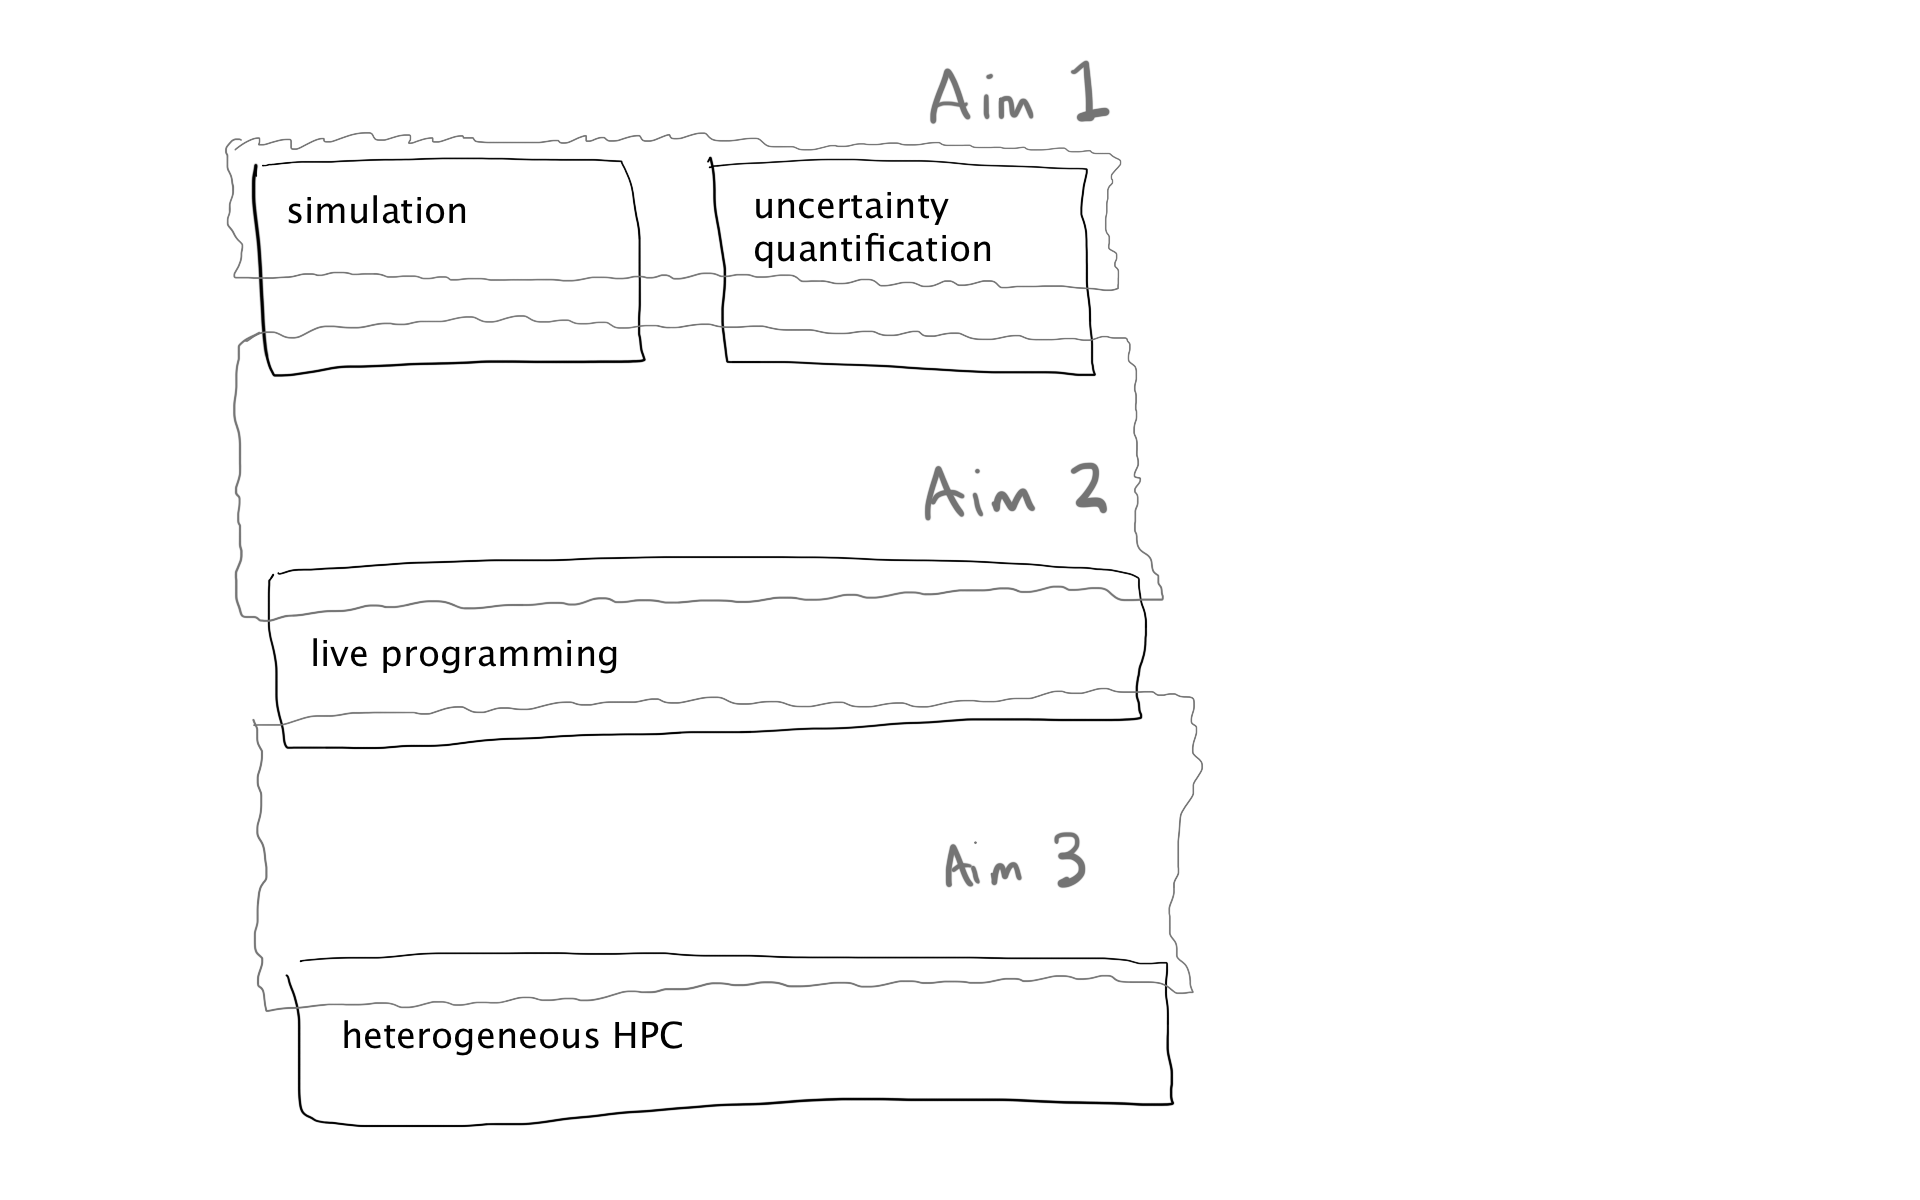
\includegraphics[scale=0.17]{figures/aims-figure.png}%
    \caption{Aims and topic areas for the project. (Note: We represent this figure in a sketch-like fashion to represent the conceptual and high-level nature of these topic areas. In reality there will be additional overlapping between them that is not shown here.)}\label{projectFig}
  \end{center}
\end{figure}

\iffalse
\tikzset{%
  block/.style    = {draw, thick, rectangle, minimum height = 3em,
    minimum width = 3em},
  sum/.style       = {draw, circle, node distance = 2.5cm}, % Adder
  splitter/.style   = {draw, circle, node distance = 2.5cm}, % splitter
}

\begin{center}
\begin{tikzpicture}[auto, node distance=2.5cm, >=triangle 45,
minimum width={width("Heterogeneous HPC")+2pt},]
\draw
    node [block, name=sim]{Simulation}
    node[block, right of=sim](uq){Uncertainty Quantification}
    node[block,below=0.1cm of sim](live){Live Programming}
    node[block,below=0.1cm of live](hpc){Heterogeneous HPC};
    
\end{tikzpicture}
\end{center}
\fi

%\begin{tikzpicture}[auto, node distance=2.5cm, >=triangle 45]
%\draw
%	node [block, name=input1] {$U$} 
%	node [sum, right of=input1] (suma1) {}
%	node [block, right of=suma1] (inte1) {$P$}
%        node [splitter, right of=inte1](split) {} 
%         node [block, right of=split] (output) {$Y$}
%         node [block, below of=inte1] (ret1) {$H$};
%    % Joining blocks. 
%    % Commands \draw with options like [->] must be written individually
%	\draw[->](input1) -- node[near end]{$b$} (suma1);
% 	\draw[->](suma1) -- node {} (inte1);
%        \draw[->](inte1) -- node {} (split);
% 	\draw[->](split) |- node {} (ret1);
% 	\draw[->](split) -- node {} (output);
%	\draw[->](ret1) -| node[pos=0.9]{$a$} (suma1);
%\end{tikzpicture}




\subsubsection*{A specific storm-surge example}
Consider the problem of predicting the maximum 
storm surge water level at a location (or locations) along a coast threatened by a cyclone. We will denote the geographical area of interest by $\Omega$ 
(the region threatened by the cyclone) and consider only 
spatial points $(x,y) \in \Omega$. We will also restrict our interest to times $t$ to an interval of time $T = [t_0, t_1]$ (the duration of the storm). 
A standard mathematical model for storm surge is provided 
by the shallow water wave equations~\parencite{tan1992shallow}
\begin{subequations}
 \label{eqn:storm} 
\begin{align}
\frac{\partial h}{\partial t} +
\frac{\partial }{\partial x} \left(uh\right) + \frac{\partial }{\partial y} \left(vh\right) -R & =  0 ,\\
\frac{\partial uh}{\partial t} +
\frac{\partial }{\partial x} \left(u^2h +  \frac12 gh^2 \right) 
+ \frac{\partial }{\partial y} \left(vuh\right) + gh \frac{\partial b}{\partial x} 
- \frac{h}{\rho} \frac{\partial P}{\partial  x} - S_{fx} - S_{wx}  &= 0 ,   \\
\frac{\partial vh}{\partial t} +
\frac{\partial }{\partial x} \left(uvh  \right) 
+ \frac{\partial }{\partial y} \left(v^2h + \frac12 g h^2 \right) + gh \frac{\partial b}{\partial y} 
- \frac{h}{\rho} \frac{\partial P}{\partial  y} - S_{fy} -  S_{wy}& = 0,  
\end{align}
\end{subequations}
%\begin{subequations}
% \label{eqn:storm} 
%\begin{align}
%h_t + \mathbf{\nabla} \cdot (h  \mathbf{u} ) - R &= 0 \\
%( \mathbf{u}h)_t + \mathbf{\nabla} \cdot \left(h \mathbf{u} \otimes  \mathbf{u}  \right)  + gh \mathbf{\nabla} (h+b) - \frac{h}{\rho}  \mathbf{\nabla} P - \mathbf{S}_f - \mathbf{S}_w &=0
%\end{align}
%\end{subequations}
where $h(x,y,t)$ is the depth of water, $u(x,y,t)$ and $v(x,y,t)$ are the $x$ and $y$ horizontal components of water velocity. In particular $h$, $u$ and $v$ are functions defined on $\Omega \times T = \mathcal{D}$. 

Here $g$ is the gravitational constant (9.81) and $\rho$ is the density of water. 
The other terms constitute input data to the model. 
The bathymetry $b(x,y)$, is the  elevation of the ocean bed.
The rate of rainfall on the region over time is $R$.
The atmospheric pressure is given by $P$ (which generates a surge due to spatial differences in atmospheric pressure associated with a large cyclone).
The $x$ and $y$ components of the frictional force generated by the flow of the surge over the ocean bed (flow over sand is different than flow through mangroves) is given by $S_{fx}$ and $S_{fy}$, respectively. 
The $x$ and $y$ components of the surface stress force (generated by the wind) is given by $S_{wx}$ and $S_{wy}$, respectively.
As is evident, there are many opportunities for uncertainty in the input  data defining this model. 

In our papers~\parencite{anugamanual,nielsen2005hydrodynamic}  these
equations and their approximation using the  AnuGA package is shown to provide a reliable
model of general flows associated with inundation due storm-surge as well as riverine flooding and tsunamis.

The parameter space $\mathcal{P}$ will represent the possible variation in the input data $R$, $b$, $P$, $S_f$, $S_w$, as well as design parameters describing actions such as raising or lowering flood barriers and releasing or diverting flow from upstream rivers, or flood basins, or indeed constructing emergency levees. 
The model solution 
$$
U_{\mathbf{p}} (\mathbf{x})  = (  h(x,y,t) , u(x,y,t) ,  v(x,y,t) )
$$
represents the water depth and velocity fields obtained by solving the model problem for a choice of parameter $\mathbf{p}$ at a particular location and time $\mathbf{x} = (x,y,t)$.
Equation~\eqref{eqn:storm} can be characterised as $M_{\mathbf{p}}(U_{\mathbf{P}}) = 0$.

In this case, the quantity of interest $Q(U_{\mathbf{p}})$ will be the maximum storm surge height at a particular location $(x_0, y_0) \in \Omega$,
$$ 
Q(U_{\mathbf{p}})  = \max_{t_0 \leq t \leq t_1} \left( h(x_0,y_0,t) + b(x_0,y_0) \right).
$$
The aim of  uncertainty quantification is to obtain useful relationships between the variations in pressure, wind and rainfall (changes of $\mathbf{p} \in \mathcal{P}$) and $Q(U_{\mathbf{p}})$, including identifying which components of the inputs  have the greatest influence on the result. 

A completely general parameter space $\mathcal{P}$ may lead to an intractable problem. It is sensible to look for a lower dimensional manifold $\mathcal{C} \subset \mathcal{P}$. This can be done algorithmically. Or in this case $\mathcal{C}$ might represent a model of the pressure, wind and rainfall associated with a cyclone of specific intensity and location. This would still involve uncertainty, and so would entail numerous solutions of our model problem to quantify the uncertainty in our quantity of interest. Finally, as we investigate our model, it might be advantageous to change the assumptions of our cyclone model, or incorporate updated forecasts or indeed play with adding different types of uncertainty to the various input data streams. This is where live programming and real time interaction with our model becomes paramount. 

%\subsubsection*{The Modelling Problem}

More formally, suppose that we have a mathematical model
$M_{\mathbf{p}}$ parameterised by the vector
$\mathbf{p}\in\mathcal{P}$. For example, $M_{\mathbf{p}}$ may be a
parameterised partial differential equation %(PPDE)
in a storm surge model. For each $\mathbf{p}$ we suppose the model is
well-defined and there exists a unique function
\begin{equation}
  \label{eq:1}
  U_{\mathbf{p}}(\mathbf{x})\, \quad \mathbf{x}\in\Omega
\end{equation}
which is a solution to the model problem, that is $M_{\mathbf{p}}(U_{\mathbf{p}})=0$.
Here the \emph{domain space} $\Omega$ represents variables such as 
time and space, 
and $U_{\mathbf{p}}$ represents scalar or vector fields of interest, 
such as storm surge water level and/or velocity.    

Sometimes the goal of the modeller is to better understand the
relationship between $\mathbf{p}$ and some lower-dimensional quantity
of interest $Q(U_{\mathbf{p}})$, such as the relationship between a
particular rainfall scenario and the maximum storm surge levels at
particular geographical locations. In order to achieve such
understanding, repeated executions of the model (or approximations of the model solution) are often required
with an expert analysis of the outputs of each stage and selection of
the next parameter set based on an assessment of those outputs. Such
repeated model executions can also be used to estimate the
\emph{uncertainty} in any given set of predictions of
$Q(U_{\mathbf{p}})$. Through the process of trying different model
parameterisations, the scientist is able to build up an understanding
of the \emph{general} relationship between $\mathbf{p}$ and
$Q(U_{\mathbf{p}})$, including the areas of the parameter space
$\mathcal{P}$ which have the greatest influence on the result and
which types of uncertainty have the greatest impact on the certainty
of the results.

\paragraph*{A specific storm-surge example:}
Consider the problem of predicting the maximum 
storm surge water level along a coast threatened by a cyclone. 
A mathematical model of storm surge is provided 
by the shallow water wave equation,  which encodes the conservation of water and Newton's second Law (Force = mass $\times$ acceleration) 
\begin{align*}
\frac{\partial h}{\partial t} +
\frac{\partial }{\partial x} \left(uh\right) + \frac{\partial }{\partial y} \left(vh\right) &= R, \\
\frac{\partial uh}{\partial t} +
\frac{\partial }{\partial x} \left(u^2h  \frac12 gh^2 \right) 
+ \frac{\partial }{\partial y} \left(vuh\right) &= - gh \frac{\partial b}{\partial x} 
+ \frac{h}{\rho} \frac{\partial P}{\partial  x} + S_{fx} + S_{wx} ,\\
\frac{\partial vh}{\partial t} +
\frac{\partial }{\partial x} \left(uvh  \right) 
+ \frac{\partial }{\partial y} \left(v^2h + \frac12 g h^2 \right) &=  - gh \frac{\partial b}{\partial y} 
+ \frac{h}{\rho} \frac{\partial P}{\partial  y} + S_{fy} + S_{wy},
\end{align*}
where $h(x,y,t)$ is the depth of water, $u(x,y,t)$ and $v(x,y,t)$ are the $x$ and $y$ horizontal components of water velocity, $g$ is the gravitational constant (9.81), $\rho$ is the density of water, $b(x,y)$ is the bathymetry (elevation of the ocean bed), $R$ is the rate of rainfall, $P$ is the atmospheric pressure (which generates a surge due to spatial differences in atmospheric pressure associated with a large cyclone), $S_{fx}$ and $S_{fy}$ are the $x$ and $y$ components of the frictional force generated by the flow of the surge over the ocean bed (flow over sand is different than flow through mangroves) , and $S_{wx}$ and $S_{wy}$ are the $x$ and $y$ components of the surface stress force (generated by the wind). As is evident, there are many opportunities for uncertainty in the data defining this model. 
As demonstrated in our papers~\parencite{anugamanual,nielsen2005hydrodynamic}  these
equations and their implementation in the AnuGA package provide a reliable
model of general flows associated with inundation due to riverine flooding, storm-surge 
and tsunamis.

The parameter space $\mathcal{P}$ needs to represent the variation in the input data $R$, $b$, $P$, $S_f$, $S_w$, as well as design parameters describing actions such as raising or lowering flood barriers and releasing or diverting flow from upstream rivers, or flood basins, or indeed constructing emergency levees. 
The domain $\Omega$ represents the variables $x$, $y$ over a geographical region and $t$ over a time interval, such as a  coastal region threatened by a cyclone over particular time interval. The model solution 
$$
U_{\mathbf{p}} (\mathbf{x})  = \begin{bmatrix} h(x,y,t) \\ u(x,y,t) \\ v(x,y,t) \end{bmatrix}
$$
represents the water depth and velocity fields obtained by solving the model problem for a particular value of the parameter $\mathbf{p}$ (or perhaps a high fidelity numerical approximation of this problem). 

A quantity of interest $Q(U_{\mathbf{p}})$ could be the maximum storm surge height at a particular location $(x_0, y_0)$
$$ 
Q(U_{\mathbf{p}})  = \max_{t_0 \leq t \leq t_1} \left( h(x_0,y_0,t) + b(x_0,y_0) \right).
$$
The aim of  uncertainty quantification is to obtain useful relationships between the variations in pressure, wind and rainfall  and $Q(U_{\mathbf{p}})$, including the which components of the inputs  which have the greatest influence on the result. 




%or to find the parameter choice $\mathbf{p}$
%which optimises $Q$. %over all $\mathbf{x}$.
%This high-level description of the ``model selection/optimisation''
% workflow 
%(shown
%graphically in Figure~\ref{fig:general-fb-loop})
 %lies at the heart of
%a great deal of modern science.
%\begin{figure}
 % \centering
  %
\includegraphics[width=.6\textwidth]{figures/general-fb-loop.pdf}
  %\caption{The human-in-the-loop modelling workflow. A scientist
    %selects an initial parameter $\mathbf{p_0}$ for their model,
    %examines the model output $Q(u_{\mathbf{p}})$, and either accepts
    %the output of the model or re-runs the model with a different
    %choice of the parameter $\mathbf{p_1}$.}
  %\label{fig:general-fb-loop}
%\end{figure}
%There are many ways of finding an optimal $\mathbf{p}$, from 
%trial-and-error experimentation to expert judgement through to fully-automated algorithmic
%optimization procedures. Often there are ways to optimise $\mathbf{p}$
%algorithmically, although these methods often introduce new parameters (the
%arguments of the function being optimised) which must be selected by the
%scientist. 
%As a result, this feedback loop will often require many
%iterations, with a scientist-in-the-loop, evaluating the results
%of the model (possibly through visualising the model output) and
%choosing a parameter update $\Delta\mathbf{p}$ at each step.
% (see
%Figure~\ref{fig:unrolled-fb-loop}). 
%Each step through this loop
%provides feedback to the scientist about the response of the system to
%a particular value of $\mathbf{p}$ --  for example, the maximum storm
%surge level under a particular rainfall scenario. 

%\begin{figure}
% \centering
%  
\includegraphics[width=\textwidth]{figures/unrolled-fb-loop.pdf}
%  \caption{If the modelling \& post-processing/visualisation steps can
%    be performed sufficiently quickly, then the scientist can explore
%    the $\mathbf{p} \rightarrow Q(u_{\mathbf{p}})$ relationship
%    \emph{interactively}, with the all the associated benefits for
%    exploratory analysis.}
%  \label{fig:unrolled-fb-loop}
%\end{figure}

From a workflow perspective, the productivity of the
modeller/scientist is proportional to the rate at which they can
explore the $\mathbf{p} \rightarrow Q(U_{\mathbf{p}})$ relationship.
Any latency improvements in this feedback loop will translate into
productivity gains~\parencite{liuEffects2014}. If the model
parameters $\mathbf{p}$ and inputs $\mathbf{x}$ are known precisely
and the quantity $Q(U_{\mathbf{p}})$ is cheap to calculate and easy to
interpret, then the task is simple: provide the scientist with an
interface for manipulating $\mathbf{p}$ and set them loose. However,
for real-world models (such as those used in flood/storm
surge/bushfire modelling) this is often not the case. There are
\textbf{three primary challenges}:
\begin{enumerate}
\item \emph{The model may not provide a way to express uncertainty in
    the inputs}. Many models do not provide methods for including
  uncertainty information in their inputs, as was the case in the 2011
  Brisbane River flood example.
\item \emph{The quantity $Q(U_{\mathbf{p}})$ may not be cheap to
    calculate}. Many
  sophisticated models require non-trivial computing resources 
  to evaluate. These compute resources may be
  difficult to secure, with submitted jobs having to wait in a queue, 
  and may
  take a long time to compute even when the resources are available.
  This is especially problematic in a disaster-response scenario,
  where an approximately correct answer provided in a short time is
  significantly more useful than a perfect answer provided after it is
  too late to act on.
\item \emph{The quantity $Q(U_{\mathbf{p}})$ together with estimates
    of its uncertainty may not be easy to interpret}. Oftentimes this
  is a visualisation problem--- the mapping
  $\mathbf{p} \rightarrow Q(U_{\mathbf{p}})$ may be high-dimensional,
  and presenting that to a decision-maker, particularly when combining
  it with its uncertainty estimates, may not be straightforward.
\end{enumerate}
%\begin{figure}
 % \centering
  %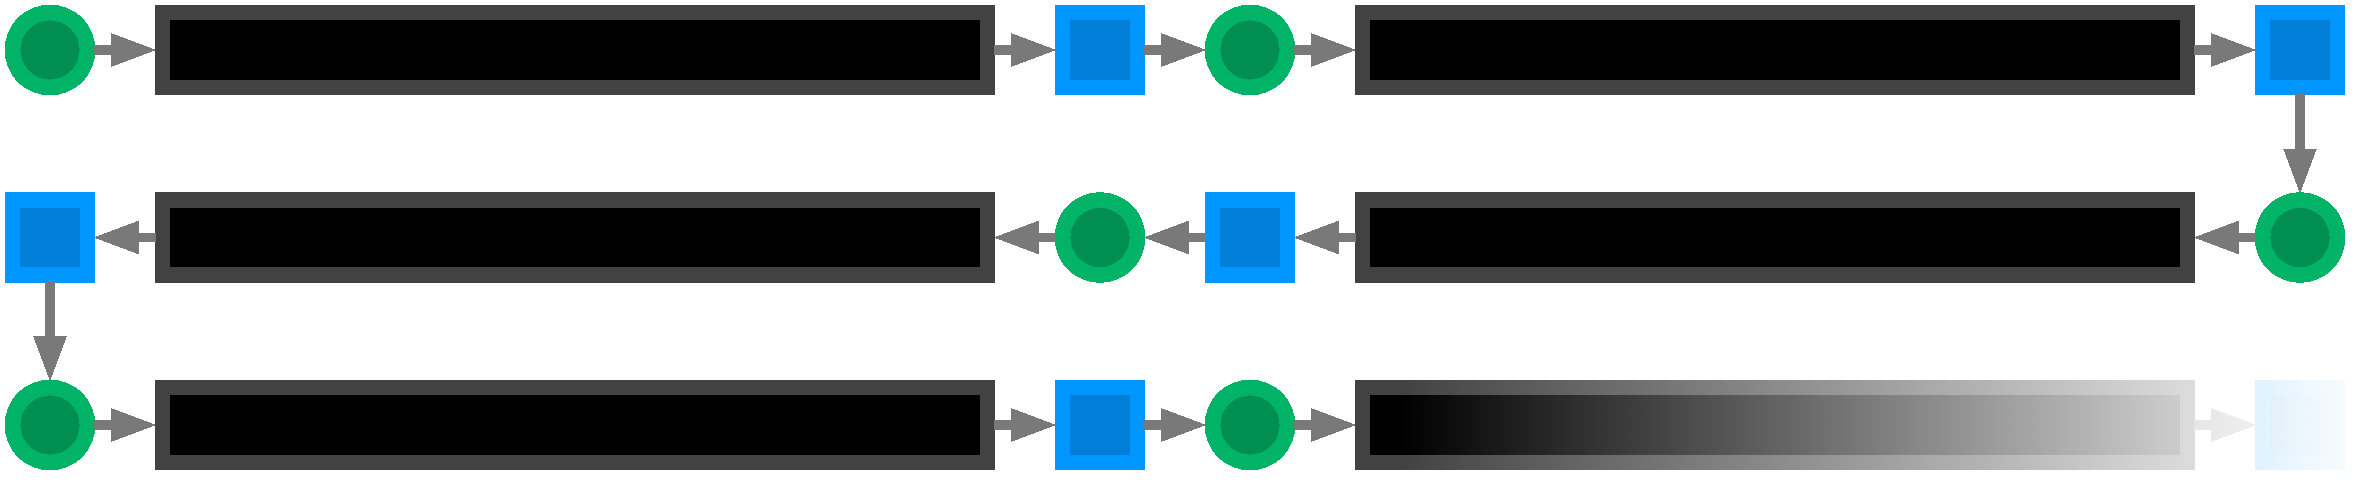
\includegraphics[width=\textwidth]{figures/long-fb-loop.pdf}
  %\caption{If the model is computationally expensive to run, then the
   % workflow is dominated by waiting for the model to finish. This
    %results in lower productivity---not only due to the time spent
    %waiting for the model, but also because of the temporal separation
  %between the selection of a new parameter $\mathbf{p}$, and seeing
 % its impact on the results of the model.}
 % \label{fig:long-fb-loop.pdf}
%\end{figure}



%\subsubsection*{Sparse-Grids and Uncertainty Quantification}

The mathematical component of this project will be based on new
developments combining sparse
grids~\parencite{BungartzGriebel2004}, reduced basis
methods~\parencite{LiebermanEtal2010,Peherstorfer2013,ChenSchwab2015,PeherstorferWillcox2015}
and uncertainty quantification. One of the main difficulties in the
study of current scientific models is the high dimensional spaces
involved, often both in the parameter and domain spaces, $\mathcal{P}$
and $\Omega$ respectively. This is a significant barrier for the
timely evaluation of models due to the `curse of dimensionality' in
which the cost scales exponentially with dimension. By using sparse
grids and reduced basis models we will be able to compute
\emph{surrogates of the full problem} which have significantly fewer
unknowns and are thus cheaper to compute whilst maintaining a high
order of accuracy. For example, a general approach would be to find a
lower dimensional manifold of the parameter space
$\mathcal{Q}\subset\mathcal{P}$ over which the model is most sensitive
using a proper orthogonal decomposition. A sparse grid surrogate of
the model over $\mathcal{Q}$ can also be computed in an offline phase,
so that in an online phase model solutions can be efficiently
estimated using the surrogate model. For many problems sparse grids
can also be used over $\Omega$ when computing solutions to the full
model to speed up the construction of a reduced basis. We will compute
sparse grid solutions via the `combination
technique'~\parencite{Griebel1990}. Figure~\ref{fig:sparse_grids}
depicts the combination technique, the equivalent sparse grid and the
corresponding full grid.

\begin{figure}
  \centering
  % Brendan: combination grid, sparse grid, fullgrid figure

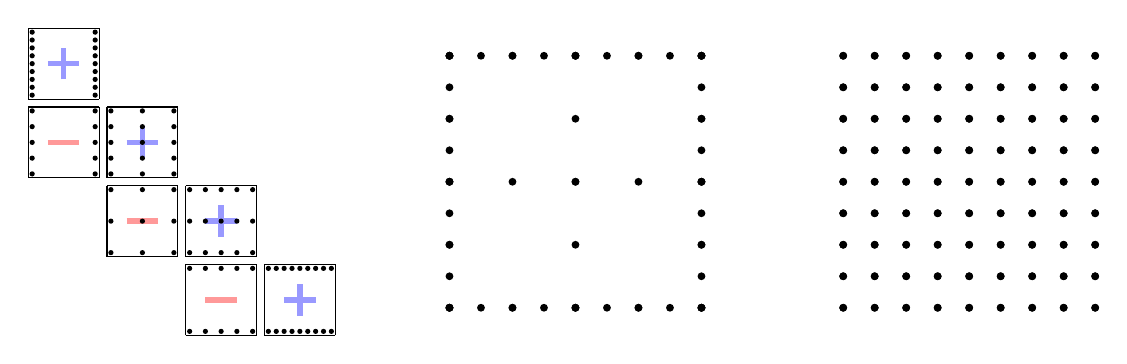
\begin{tikzpicture}%[scale=0.8]
%\scriptsize
%%% Draw squares around component grids
\foreach \i in {1,...,4}
{
	\pgfmathtruncatemacro{\x}{(\i - 1)};
	\draw[] (0.05+1.0*\x, 3.05-1.0*\x) -- (0.05+1.0*\x+0.9, 3.05-1.0*\x) {};
	\draw[] (0.05+1.0*\x, 3.05-1.0*\x) -- (0.05+1.0*\x, 3.05-1.0*\x+0.9) {};
	\draw[] (0.05+1.0*\x+0.9, 3.05-1.0*\x) -- (0.05+1.0*\x+0.9, 3.05-1.0*\x+0.9) {};
	\draw[] (0.05+1.0*\x, 3.05-1.0*\x+0.9) -- (0.05+1.0*\x+0.9, 3.05-1.0*\x+0.9) {};
	%%% optional plotting of coefficients
	\draw[blue!40,line width=0.7mm] (0.5+1.0*\x-0.2, 3.0+0.5-1.0*\x) -- (0.5+1.0*\x+0.2, 3.0+0.5-1.0*\x);
	\draw[blue!40,line width=0.7mm] (0.5+1.0*\x, 3.0+0.5-1.0*\x-0.2) -- (0.5+1.0*\x, 3.0+0.5-1.0*\x+0.2);
}
\foreach \i in {1,...,3}
{
	\pgfmathtruncatemacro{\x}{(\i - 1)};
	\draw[] (0.05+1.0*\x, 2.05-1.0*\x) -- (0.05+1.0*\x+0.9, 2.05-1.0*\x) {};
	\draw[] (0.05+1.0*\x, 2.05-1.0*\x) -- (0.05+1.0*\x, 2.05-1.0*\x+0.9) {};
	\draw[] (0.05+1.0*\x+0.9, 2.05-1.0*\x) -- (0.05+1.0*\x+0.9, 2.05-1.0*\x+0.9) {};
	\draw[] (0.05+1.0*\x, 2.05-1.0*\x+0.9) -- (0.05+1.0*\x+0.9, 2.05-1.0*\x+0.9) {};
	%%% optional plotting of coefficients
	\draw[red!40,line width=0.7mm] (0.5+1.0*\x-0.2, 2.0+0.5-1.0*\x) -- (0.5+1.0*\x+0.2, 2.0+0.5-1.0*\x);
}
%%% Combination grids
\foreach \i in {1,...,18} %2*9
{
	\pgfmathtruncatemacro{\y}{(\i - 1) / 2};
	\pgfmathtruncatemacro{\x}{\i - 1 - 2 * \y};
	\node[fill,circle,scale=0.2] at (0.1+0.8*\x,3.1+0.1*\y) {};
	\node[fill,circle,scale=0.2] at (3.1+0.1*\y,0.1+0.8*\x) {};
}
\foreach \i in {1,...,15} %3*5
{
	\pgfmathtruncatemacro{\y}{(\i-1)/3};
	\pgfmathtruncatemacro{\x}{\i-1-3*\y};
	\node[fill,circle,scale=0.2] at (1.1+0.4*\x,2.1+0.2*\y) {};
	\node[fill,circle,scale=0.2] at (2.1+0.2*\y,1.1+0.4*\x) {};
}
\foreach \i in {1,...,10} %2*5
{
	\pgfmathtruncatemacro{\y}{(\i-1)/2};
	\pgfmathtruncatemacro{\x}{\i-1-2*\y};
	\node[fill,circle,scale=0.2] at (0.1+0.8*\x,2.1+0.2*\y) {};
	\node[fill,circle,scale=0.2] at (2.1+0.2*\y,0.1+0.8*\x) {};
}
\foreach \i in {1,...,9} %3*3
{
	\pgfmathtruncatemacro{\y}{(\i - 1) / 3};
	\pgfmathtruncatemacro{\x}{\i - 1 - 3 * \y};
	\node[fill,circle,scale=0.2] at (1.1+0.4*\x,1.1+0.4*\y) {};
}
%%% Sparse grid
\foreach \i in {1,...,18} %2*9
{
	\pgfmathtruncatemacro{\y}{(\i - 1) / 2};
	\pgfmathtruncatemacro{\x}{\i - 1 - 2 * \y};
	\node[fill,circle,scale=0.3] at (5.4+3.2*\x,0.4+0.4*\y) {};
	\node[fill,circle,scale=0.3] at (5.4+0.4*\y,0.4+3.2*\x) {};
}
\foreach \i in {1,...,15} %3*5
{
	\pgfmathtruncatemacro{\y}{(\i-1)/3};
	\pgfmathtruncatemacro{\x}{\i-1-3*\y};
	\node[fill,circle,scale=0.3] at (5.4+1.6*\x,0.4+0.8*\y) {};
	\node[fill,circle,scale=0.3] at (5.4+0.8*\y,0.4+1.6*\x) {};
}
%%% Full grid
\foreach \i in {1,...,81} %9*9
{
	\pgfmathtruncatemacro{\y}{(\i - 1) / 9};
	\pgfmathtruncatemacro{\x}{\i - 1 - 9 * \y};
	\node[fill,circle,scale=0.3] at (10.4+0.4*\x,0.4+0.4*\y) {};
	\node[fill,circle,scale=0.3] at (10.4+0.4*\y,0.4+0.4*\x) {};
}
\end{tikzpicture}  
  \caption{Combination grids on the left (with coefficients, marked with
    a blue plus for $+1$ and red minus for $-1$), sparse grid in the
    middle, full grid on the right. Note the marked reduction in the number of 
    grid points for the sparse grid relative to the full grid. 
   This is even more pronounced in higher dimensions.}
  \label{fig:sparse_grids}
\end{figure}

Propagating uncertainty in scientific models which are high
dimensional and/or expensive to compute is a significant challenge.
For models which are not stochastic in nature, and thus have no means
of directly quantifying uncertainty, one must typically estimate
statistical moments via Monte Carlo methods or quadrature rules. For
high dimensional problems it has been shown that sparse grids can
estimate these moments faster and more accurately than traditional
Monte Carlo methods when the probability density functions are
sufficiently
smooth~\parencite{JakemanRoberts2013,FranzelinDiehlPfluger2014}.
Despite the advantages of reduced basis methods, the manifold
$\mathcal{Q}$ is still sufficiently high dimensional that the
quantification of uncertainty remains a challenge due to the sheer
number of function evaluations required. This is particularly true
when the quantification of uncertainty in a model is a component of an
optimisation algorithm. As such it is important to continue to
develop efficient numerical methods for uncertainty quantification
for high dimensional problems. Replacing the full model with a reduced
basis model also adds additional error and uncertainties. One needs to
have some idea what the model outcomes may be for parameters not lying
on the lower dimensional manifold $\mathcal{Q}$. An important part of
developing reduced models is `verifying' the model, by bounding their
error of the surrogate for example. By using ensemble methods,
multifidelity models~\parencite{NgWillcox2014} and gradient enhanced
approximation~\parencite{deBaarHarding2015,Jakeman2015} we hope to
improve the verification and propagation of uncertainties in models.
Incorporating ideas from `Kriging' (Gaussian process regression), a
feature of which is having confidence intervals over an interpolant,
together with sparse-grid interpolation, we will be able to express
uncertainties explicitly in the surrogate model.



%\subsubsection*{Live Coding of Scientific Simulation}

\iffalse
Live coding is a term which has been used to denote systems which
support the direct intervention of the programmer in a program's
run-time state. It can be thought of as an extreme version of the
agile programming methodology~\parencite{fowlerAgile2001}, where
code changes are hot-swapped into running programs, allowing for
extremely fast exploration and iteration of new ideas and system
updates. As the ambition of live-coding has grown, support systems and
languages have evolved to, for example, create, modify and interact
with music and hardware devices in real time. Such an approach has
been termed `\emph{with-time}
programming'~\parencite{sorensen2010programming}. 
\fi

This project will
make use of the \emph{Extempore} software
environment\footnote{\url{http://extempore.moso.com.au}} which has
been used for live modification and real-time visualisation of
particle-in-cell (PIC) plasma physics simulation codes, with
negligible performance overhead compared to batch-mode execution in
C~\parencite{swiftLive2016}. This allows the scientist to modify the
domain size/shape, the initial and boundary conditions, and various
other parameters while the simulation is running, with live visual
feedback.

The Extempore software environment is a key tool for this project as
it allows us to fine tune our suite of simulation software for the
specific requirements of the task domain.




\subsubsection*{Live Coding for Uncertainty
  Quantification}

This project will
make use of the \emph{Extempore} live-coding software
environment.%\footnote{\url{http://extempore.moso.com.au}}
 Extempore has already
been used for the live modification and real-time visualisation of
particle-in-cell plasma-physics simulation codes with
negligible performance overhead compared to batch-mode execution in
C~\parencite{swiftLive2016}. 



Such a live deployment of a traditional, batch-oriented HPC simulation allows a user to 
modify the
domain size and shape, the initial and boundary conditions, and various
other parameters of a simulation while that simulation is running. It is of use
for optimising software for later, stand-alone,
deployment as well as for harnessing and steering simulation codes
after deployment.

%The Extempore software environment is a key tool for this project as
%it allows us to fine tune our suite of simulation software for the
%specific requirements of the task domain.

The ability to stop, modify, or restart computations `in flight' has
the potential to significantly improve the efficiency of an
uncertainty analysis. There exist many algorithms, for example
adaptive Markov chain Monte Carlo methods~\parencite{GilksEtal1994}, 
which attempt to choose the best samples based on the sampling
history. For complex problems however, a domain expert
may often have
a better idea about the region of the parameter domain where function
evaluations should be concentrated. Through live programming within a
tight feedback loop a domain expert can incrementally guide the
current sampling strategy being used for uncertainty 
quantification, and in turn be guided by 
real time information derived from the reduced order model 
(such as surpluses
provided by sparse grid approximation to 
identify important parameter dimensions and regions of interest), 
to improve the end result. The resulting strategies are expected to be
more aggressive in nature as they are better targeted to the specific
problem at hand. The result of this should be more efficient quantification of
uncertainty.

In this project, using live coding to accelerate the feedback loop between the vector of input parameters,
$\mathbf{p}$,  and quantities of interest  will give a scientist the ability to interactively
\emph{explore} the connection (and the associated uncertainty) between
the different dimensions of $\mathbf{p}$ and the overall response of
the system. Such a prototyping and optimising of these models ({\bf Aim 2 of our project}) will help us rapidly scope and deliver 
robust models. The ``liveness'' that this approach brings will also be deployed 
into the uncertainty quantification models. For example, reduced-basis methods for uncertainty 
quantification typically employ a number of ``offline'' simulations that are used together with an ``online'' simulation of 
a system of interest to provide uncertainty estimates for that online simulation; we will apply novel live-coding
approaches to such methods where the offline as well as the online simulations are all harnessed and live. The 
potential advantage of such an approach is that the offline simulations can be restarted, modified, reduced and 
explored at the same time that the online simulation is running. Such a research agenda in live coding is one that 
includes human-computer interaction (HCI) as well as software engineering. HCI research questions include the realistic time-scales of 
human-in-the-loop interaction with running simulation software, both for software development and for decision making in real time.
HCI research methodologies will include ethnographic studies and protocol analysis of ``staged'' interaction scenarios including
human actors. We will be looking to identify states of interaction 
of expert users with our live-coding systems as well as transitions between them -- much as we have already done so in the 
context of computer music~\parencite{swift2014coding}.






%This will be used to {\bf rapidly prototype software} with a view to 
%dentifying the necessary interactive controls needed to modify and interact with 
%the final, relased and running, software in real-time. 
%By understanding the human-factors and systems-level time
%constraints on the delivery of useful information in disaster-response
%settings, we will also be able to specify timing requirements on our model
%simulations as in the next section. 
%By developing software that is time-constrained and
%time-aware, we will be able to provide decision makers with
%information when it is needed and with an estimate on the uncertainty
%of that information.
%Ultimately, the scientist needs an \textbf{interactive interface} for
%gleaning insights from their models in the presence of these
%challenges.
%\newpage

%\begin{figure}
 % \centering
  %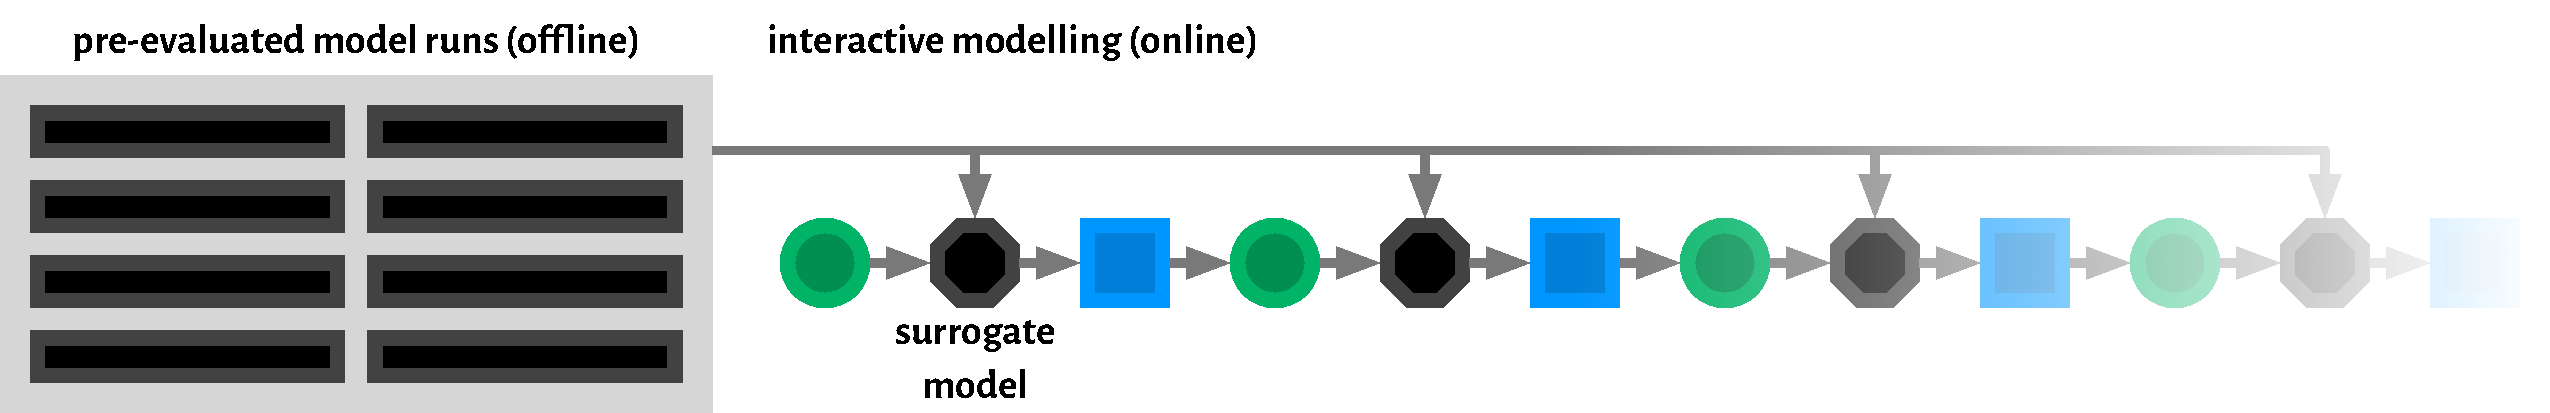
\includegraphics[width=\textwidth]{figures/sg-surrogate-model-fb-loop.pdf}
  %\caption{Using the sparse grids and reduced basis models, the computationally
   % expensive model calculations can be done ahead-of-time and used to
    %construct a surrogate model which can be used to re-claim the
    %interactive workflow of Figure~\ref{fig:unrolled-fb-loop}}.
  %\label{fig:sg-surrogate-model-fb-loop}
%\end{figure}

%Impact: new algorithms, software, high performance computer systems
%and visualisation techniques for time-bound environmental simulation
%with uncertainty. New software tools for the simulation of flood
%surges and tsunami. New methodologies for rapid and agile software
%development and usability using live programming. New knowledge of
%human-in-the-loop requirements for support systems in the context of
%environmental disaster management. New algorithms, software, high
%performance computer systems and visualisation techniques for
%time-bound environmental simulation with uncertainty. New software
%tools for the simulation of flood surges and tsunami. New
%methodologies for rapid and agile software development and usability
%using live programming. New knowledge of human-in-the-loop
%requirements for support systems in the context of environmental
%disaster management.





%\subsubsection*{From Disaster-Response Human-Factors Optimisation to Software Development}

% GOMS model for co-operative scenarios where someone wants
% information, and someone is trying to present it to them

% it's about chunking complex tasks c.f. beginning-middle-end

% the goal: quantitative requirements on the time bounds, which has
% implications for the design of the systems

Similar to ~\parencite{ramchurn2016human} we will employ game
scenarios to understand and optimise collaboration for disaster
response~\parencite{ramchurn2016human}. However, our focus will be on
decision-maker/modeller communication rather than human/agent
communication and our game scenarios will take place while software
and systems parameters, particularly the human-computer interface,
visualisations and system configuration, are being tuned in real time
by a live coder. In a novel approach, the protocols obtained from this
live coding will then be analysed to determine macro ``chunking''
states, of human action and transitions between those states. We have
recently used similar approaches to understand the real-time actions
of single live-coders in computer music
performance~\parencite{swift2014coding} and the macro-gesture states
of group computer musicians using
iPads~\parencite{martin2015tracking}. In both of these studies,
transition matrices derived from interaction protocols were able to
yield insights into the artistic process. In the case of the present
project, data from the interaction protocols of the live-coder will be
feed back into redesign of the software interface and the controls
needed for the computational platform.

By way of one simple example, we imagine that, perhaps, the live coder
finds that a particular measure of uncertainty, \emph{measure-A}, is
routinely requested by a decision maker after another particular
measure, \emph{measure-B}. The live coder could tune up the software
in real time so that these two measures could be presented together.
The interaction protocols in this instance might reveal insights into
the \emph{context} where these two measures were requested one after
the other and the software might be redesigned to recognise that
context and to make the two measures accessible in that context. For
another simple example, the live-coding protocol might show that data
processing needed to be occasionally shifted from one part of a cloud
resource to a local cluster. Examination of these instances could
impact on the computer systems settings needed to properly deploy
these simulations. Our approach to protocol analysis will go well
beyond simple examples like these and will use matrix theory to derive
insights into the nature of state transitions across entire protocols
and across test participants.



%\subsubsection*{Interactive Design Optimisation}

The methodology we will develop for this project will also have
significant benefits for engineering design. We will explore this in
the context of design optimisation problems from aerospace and
aeronautics. Design optimisation poses a significant challenge due to
the large number of input parameters, for example in describing the
geometry of an airfoil, and there are a number of ways in which
uncertainty comes into the modelling. For example, the manufacturing
process is not exact, and the full range of attack angles, velocities,
stresses and weather conditions the airfoil will be exposed to during
flight can only be guessed at. In this project we will build on our
previous work in applying sparse grid methods in airfoil
design~\parencite{SU2,deBaarHarding2015}, using an interactive
feedback loop to improve the efficiency of the design process within
our live coding and uncertainty quantification framework.




\subsubsection*{High-Performance Computing Systems Support}

A reliance on high performance computing for the evaluation of
scientific models provides additional challenges to the technical side
of the project. Specifically, our algorithms must be highly scalable
and robust to errors and faults in the computer system layer. There
have been many recent developments in both highly-scalable algorithms
and the sparse grid combination technique \cite{sgctalg15,pdsec15extsgctalg} 
which will be of use for
this and, additionally, it has been recently shown that such
computations can be made
robust~\parencite{HardingHLS2015,AliEtal2015,Ali11022016}. By leveraging and
continuing to develop these algorithms we can ensure that the
offline components of our software system that require high performance
computing resources will be both scalable and robust.

In this project we will leverage on-demand compute resources, such as
the Amazon AWS cloud~\parencite{amazonAws} and the National Compute
Infrastructure NCI Cloud~\parencite{nciCloud}. Using these cloud
services will further improve the project's ability to deliver timely
results in high-pressure and time-critical decision making scenarios.

Once again, we emphasise that our approach to live coding of test
software is a novel aspect of our methodology. The \emph{Extempore}
tool that we have developed has been shown to be able to harness and
steer scientific simulation in real time. In this part of the project,
we will apply this tool to the real-time steering of the computer
systems layer itself.

This will involve developing code libraries to assist the developer in
the live performance evaluation and tuning of these complex and highly
parallel simulations. For example, groups of processes will be
allocated to different parts of the simulation. If some parts are
delayed relative to others, processes can be `stolen' from the faster
group to improve load balance \cite{parSGCT16}. Communication
bottlenecks can be identified and alternate communication algorithms
can be employed to rectify this.  Different computational kernels can
be selected depending on the current memory system and floating point
performance.  It should be noted that this fine-tuning is not only
application-dependent, but within an application, it depends on the
workload selected, and even within that, may depend on the current
phase of the simulation. Only Live Programming by \emph{Extempore} has
the flexibility and agility to facilitate such a degree of performance
tuning.


%\subsubsection*{Other projects}

The two postdoctoral fellows and three of the five PhD students 
will be concerned with the main aims of this grant application: One postdoctoral fellow and one PhD student in 
Mathematics will study storm surge equations in realistic topographies with the calculation of uncertainty. They will work closely with the other postdoctoral fellow 
and one PhD student in Computer Science to study the application of live coding to uncertainty quantification of these equations. The third
PhD student will work with the postdoctoral fellow in Computer Science to study  live coding of the HPC infrastructure for these systems.

The remaining two PhD students will study other aspects of the overall context shown in Figure 1. One PhD student in Mathematics will study other environmental models of relevance
to disaster management such as ..... The other PhD student will study the human-computer-interaction context of real-time disaster management. 
Similar to the impact of visually presented geodata on decision
making~\parencite{kinkeldey2015evaluating}, the particular
visualisations of uncertainty in our environmental models will need to
be systematically evaluated with human participants. Here we will
adopt traditional human-factors trials with non-expert participants
together with qualitative feedback from emergency services experts. We
will solicit qualitative feedback from expert participants from
emergency authorities in our local area including ACT Emergency
Services, Geosciences Australia, the Australian Maritime and Safety
Authority and the Australian Federal Police. Perspectives offered by
this participant pool will be important in extrapolating our study
results to real world disaster-management.

We also anticipate a number of Honours and other student projects concerned with the overall context of our research.



 





\noindent{\bf International collaboration: }
We have already mentioned the active collaboration that we have with researchers at Sandia laboratories in the USA. Uncertainty Quantificaion is a topic of very great interest in the computational science community. Our very novel approach to this problem involving live coding is bound to generate huge interest and further opportunities for international collaboration as this project progresses. Already we have delivered one invited workshop on the Extempore system at the major SC conference in Austin, TX in 2015. \\

\noindent{\bf Dissemination:}
We describe plans for publication below. 
As discussed in the project description and under feasibility, we plan to establish contact with disaster management agencies to scope the human interface needs of users and to engage emergency services personnel as human participants in live-coding experiments. This industry engagement will disseminate our work to these stakeholders and will hopefully lead to downstream collaborations over time.

Our research in this proposal has been framed around fundamental problems that address the three main aims of the project. The core scientific objectives of each aim will be able to be achieved with reduced models, making them clearly realisable within the three year timeframe. As time permits, our objective is to make our simulations as close to the real-world as possible, including the use of realistic topographic data for flood simulations. This greater realisim is bound to generate much interest in the media and the community. Arising from this interest, we envision that many future projects may involve active collaboration with emergency services and industry (including computer systems providers). 


%\subsubsection*{Interactive Visualisation of Environmental Forecasts with Uncertainty}

Similar to the impact of visually presented geodata on decision
making~\parencite{kinkeldey2015evaluating}, the particular
visualisations of uncertainty in our environmental models will need to
be systematically evaluated with human participants. Here we will
adopt traditional human-factors trials with non-expert participants
together with qualitative feedback from emergency services experts. We
will solicit qualitative feedback from expert participants from
emergency authorities in our local area including ACT Emergency
Service, Geosciences Australia, the Australian Maritime and Safety
Authority and the Australian Federal Police. Perspectives offered by
this participant pool will be important in extrapolating our study
results to real world disaster-management.



\iffalse
The overall context of our project is shown in
Figure \ref{fig:projcontect}.  . In the application layer, the project
is concerned with developing and delivering simulations with
quantified uncertainty in a time-bound manner under conditions of
rapidly changing human demands. At the systems layer, the project is
concerned with managing large and ambitious simulations, and their
associated data, in emergency disaster management settings where the
very existence of such systems may be volatile. Both of these layers
of concern will be supported by a novel live-coding approach to
software development and prototyping as well as the use of live-coding
for delivered simulations in order to modify and tune them, and their
computational systems in real time.



\begin{figure}
% insert Henry's photo here?
\caption{The overall system context of the project}
\label{fig:projcontect}
\end{figure}

\fi
\iffalse
%move this stuff into benefits?

\subsubsection*{Expected Outcomes}

This project will provide the following discoveries:
\begin{enumerate}

\item a suite of interactive, real-time modelling tools for
  surge-tsunami flood disasters which combine high fidelity
  simulations (fine grids) with low fidelity (coarse grid) simulations
  to quantify uncertainty, optimised for human exploration

\item a `live software engineering' approach to the development,
  deployment and optimisation of these interactive software systems

\item models of group interaction scenarios for decision-making with
  expert modelling support; from these models, we will obtain
  empirical estimates of the time constraints that such scenarios
  impose on software and computer system requirements and the live
  controls needed to run them effectively in volatile contexts

\item interactive information visualisation of simulation predictions
together with uncertainties


\end{enumerate}
\fi


\subsection*{BENEFIT}


Solutions to the core scientific problems of the three main aims of our project will be of high impact and will lead to the future development of  software infrastructure for disaster modelling including the quantifying of uncertainty. As noted above, we anticipate being able to use other funding to add several PhD students, and other project students, to the project team and this larger team will take the entire project in the direction of building actual deliverable software. This larger team will also provide very good value to the ARC in terms of funds invested. Together with the in-kind contributions to the project, we assess in our budgeting that an ARC investment of \$x will buy \$y worth of research effort.
  As also discussed, we plan to establish contact with disaster management agencies to scope the visualisation and human interface needs of users. 

In a world that is prey to a large number of environmental risks,
the societal benefit of improved computational modelling for disaster management is huge.
This project addressess the mathematical challenges (through new approaches
to uncertainty quantification) and the software development challenges (through live coding
 for rapid prototyping) and the systems support challenges (coping with volatile and 
 rapidly changing systems environments) of one aspect (flood inundation) of this very important area.
 
In addition to the academic benefits of the research program described here, there are potential industrial benefits
through the seeding of enterprises that develop and deliver guaranteed modelling infrastructure to disaster management
agencies.

\iffalse
This research is aims to unlock the power of sophisticated
computational simulation incorporating uncertainty for
\emph{interactive} use.  Although we concentrate our research on
simulation support for disaster response, the ultimate potential of
this work is to eventually empower domain experts from a broad range
of areas to better use the high-performance computing power which is
now available to them. We envision a future where performing a complex
flood model or disaster simulation is as interactive and \emph{alive}
as flicking through photos on a tablet.\\



There are several benefits arising from the successful completion of
this project. They include, economic, societal as well as
environmental along with the generation of new knowledge:
\begin{itemize}
\item Reduced economic losses from disasters such as flooding
\item Reduced property damage from disasters
\item Reduced loss of life from disasters
\item New knowledge in the understanding of disaster modelling, and
  hence forecasting.
\end{itemize}
\fi

\subsection*{RESEARCH ENVIRONMENT}
% - Outline the adequacy and opportunities within the Research Environment in your relevant department, school or research group, and the extent to which it will provide for knowledge growth, innovation, collaboration, mentoring and student training
% - Describe the existing, or developing, research environment within the Administering Organisation and collaborating Organisation(s) which will enable this Project
% - Describe how the Project aligns with the Administering Organisation’s research plans and strategies.

The Australian National University is a research-intensive university
of high international standing. The quality of the research at ANU has
been reflected in every one of the ERA evaluation exercises where,
relevant to the current proposal, both Information and Computing
Sciences (08) and Mathematical Sciences (01) have been assessed as
being at the highest level of 5. At ANU, the Research School of
Computer Science and the Mathematical Sciences Institute have a long
and deep collaboration in numerical and applied mathematics, notably
in a number of ''Area'' projects linked to the supercomputing
facilities on campus. Indeed, since the early 1980s ANU has housed the
largest supercomputers in Australia and the present National
Computational Infrastructure is located on campus.

Over the next 2 years, a new building will be constructed at ANU to
locate the Mathematical Sciences Institute with part of the Research
School of Computer Science. This co-location of academics in these two
areas will be particularly fruitful for the present project. Indeed,
it is possible that this project will become a showcase of cooperation
between these two Schools and that some of the more visible and
interactive components of the project will be strongly featured in
outreach activities.

Furthermore, the cloud computing facilities at the NCI National
facilities will provide an ideal testbed for the
project. Virtualization is necessary for tuning Extempore, and the
size of the clusters will permit large-scale simulations by project
staff.


\subsection*{COMMUNICATION OF RESULTS}
% - Outline plans for communicating the research results to other researchers and the broader community, including but not limited to scholarly and public communication and dissemination.

The ANU expects publications at the highest levels of international
journals and conferences. We will communicate the results of this
project by publishing in top venues such as the ``SIAM Journal of
Scientific Computing'',``Parallel Computing'', and the ``Journal of
Computational Science''. In computer science, refereed publications
associated with the top conferences are more prestigious than
journals. Our publication targets will be the ACM Conference on Human
Factors in Computing Systems (CHI), OOPSLA, ICSE, VL/HCC,
Supercomputing (SC), IEEE International Parallel and Distributed
Processing Symposium (IPDPS), Computer Supported Cooperative Work
(CSCW) and IEEE Information Visualisation. In both disciplines, we
also value the community and high quality of Australian conferences,
and we will be submitting work to OzCHI, ASWEC and Computational
Techniques and Applications (CTAC).


In addition, the source code contributions of this project will be
released to the public. Both the Extempore live programming system
(\url{https://github.com/digego/extempore}) and the AnuGA shallow
water simulation package
(\url{https://github.com/GeoscienceAustralia/anuga_core}) are
available on GitHub under MIT and GPLv2 licences respectively.
Parallel Sparse Grid Combination codes are available from CI
Strazdins' website.  We are committed to accessible and reproducible
computational science, and support these goals by using free software
licences and developing our code in the open on GitHub.



\subsection*{MANAGEMENT OF DATA}
% - Outline plans for the management of data produced as a result of the proposed research, including but not limited to storage, access and re-use arrangements.
% - It is not sufficient to state that the organisation has a data management policy. Researchers are encouraged to highlight specific plans for the management of their research data.

All research output will be stored on the ANU Data Commons and ANU
Digital Collections.

Data Commons is a central data repository for ANU research data which
has been designed to securely store data and ensure that data are
immune to format and media changes. This repository enables data to be
accessed and reused with full open-access functionality to the public.

Digital Collections accepts journal articles, conference papers, book
chapters, working or technical papers and other forms of scholarly
communication. It is also a repository for digital images of
manuscripts and photographs in other university research collections.



\fontsize{10}{15}\selectfont
\bibliographystyle{plain}
\bibliography{references}
%\subsection*{REFERENCES}

\vskip -2.5em
% \printbibliography[title=\ ]



\end{document}

% Local Variables:
% TeX-engine: xetex
% End:
